\selectlanguage{italian}

\section{Proprietà generali}

La forma tipica di una reazione nucleare è la seguente:
\begin{equation*}
	\mathrm{a} + \mathrm{X} \rightarrow \mathrm{Y} + \mathrm{b}
\end{equation*}
dove $ \mathrm{X} $ e $ \mathrm{Y} $ sono nuclidi target-like, $ \mathrm{a} $ e $ \mathrm{b} $ projectile-like. Una scrittura alternativa è: $ \mathrm{X} \left( \mathrm{a},\mathrm{b} \right) \mathrm{Y} $.\\
In linea generale, le reazioni nucleari soddisfano alcune leggi di conservazione, sebbene alcune di esse non in maniera sempre esatta: energia totale, momento lineare totale, momento angolare totale, carica elettrica totale, parità, numero atomico. In base all'energia per nucleone possono presentarsi comportamenti aggiuntivi:
\begin{enumerate}
	\item low-energy ($ E \lesssim 10\mev $ per nucleone): non ci sono processi legati all'interazione forte, dunque si conservano anche il numero di protoni e quello di neutroni;
	\item medium-energy ($ 100\mev \lesssim E \lesssim 1\gev $ per nucleone): subentrano processi di meson production, dunque protoni e neutroni possono trasformarsi gli uni negli altri;
	\item high-energy ($ E \gtrsim 10\gev $ per nucleone); possono essere prodotte molte particelle esotiche, arrivando a riarrangiare anche i quarks nei nucleoni.
\end{enumerate}
Inoltre, dato che affinché avvenga la reazione si deve superare la barriera coulombiana nei nuclei, è necessario che la reazione abbia un certo $ Q $-value. Dalla conservazione dell'energia totale si ha:
\begin{equation*}
	M_{\mathrm{a}} c^2 + T_{\mathrm{a}} + M_{\mathrm{X}} c^2 + T_{\mathrm{X}} = M_{\mathrm{Y}} c^2 + T_{\mathrm{Y}} + M_{\mathrm{b}} c^2 + T_{\mathrm{b}}
	\quad \Rightarrow \quad
	Q = M_{\mathrm{a}} c^2 + M_{\mathrm{X}} c^2 - \left( M_{\mathrm{Y}} c^2 + M_{\mathrm{b}} c^2 \right)
\end{equation*}
Se $ Q > 0 $ si parla di \textit{reazione esoergonica} (o esotermica), nella quale parte della massa nucleare o della binding energy viene liberata sotto forma di energia cinetica, mentre se $ Q < 0 $ di \textit{reazione endoergonica} (o endotermica), nella quale parte dell'energia cinetica è convertita in massa nucleare o binding energy. Nel caso in cui $ Q = 0 $ si parla di \textit{collisione elastica}.\\
Una reazione è sempre possibile se $ Q \ge 0 $, mentre se $ Q < 0 $ è necessario che $ T_{\mathrm{a}} $ superi una certa threshold energy:
\begin{equation}
	T_{\text{th}} = -Q \frac{M_{\mathrm{Y}} + M_{\mathrm{b}}}{M_{\mathrm{Y}} + M_{\mathrm{b}} - M_{\mathrm{a}}}
	\label{eq:6.1}
\end{equation}
Dalla conservazione dell'impulso, invece, considerando il laboratory frame in cui il target $ \mathrm{X} $ è a riposo e definendo $ \theta $ e $ \xi $ gli angoli tra i momenti di $ \mathrm{Y} $ e $ \mathrm{b} $ e quello di $ \mathrm{a} $, si ha:
\begin{equation*}
	\begin{cases}
		p_{\mathrm{a}} = p_{\mathrm{b}} \cos \theta + p_{\mathrm{Y}} \cos \xi \\
		0 = p_{\mathrm{b}} \sin \theta - p_{\mathrm{Y}} \sin \xi
	\end{cases}
\end{equation*}
Si hanno tre equazioni in quattro incognite ($ T_{\mathrm{b}}, T_{\mathrm{Y}}, \theta, \xi $), dunque non c'è soluzione unica. Dato che è più facile osservare $ \mathrm{b} $ rispetto ad $ \mathrm{Y} $, dato che quest'ultimo può rimanere all'interno dello strato target, conviene eliminare le osservabili relative ad $ \mathrm{Y} $, trovando:
\begin{equation}
	\sqrt{T_{\mathrm{b}}} = \frac{1}{M_{\mathrm{Y}} + M_{\mathrm{b}}} \left[ \sqrt{M_{\mathrm{a}} M_{\mathrm{b}} T_{\mathrm{a}}} \cos \theta \pm \sqrt{M_{\mathrm{a}} M_{\mathrm{b}} T_{\mathrm{a}} \cos^2 \theta + \left( M_{\mathrm{Y}} + M_{\mathrm{b}} \right) \left( M_{\mathrm{Y}} Q + (M_{\mathrm{Y}} - M_{\mathrm{a}}) T_{\mathrm{a}} \right)} \right]
	\label{eq:6.2}
\end{equation}
Si può quindi calcolare $ T_{\mathrm{b}} $ in base alla misura dell'angolo $ \theta $.\\
In Fig. \ref{reac-graph} è riportato il plot di $ T_{\mathrm{b}} $ rispetto a $ T_{\mathrm{a}} $ a vari angoli $ \theta $ per la reazione $ \ch{^3H} \left( p,n \right) \ch{^3He} $, la quale ha $ Q = -763.75\kev $: si può notare che quasi ovunque c'è una corrispondenza biunivoca tra $ \theta $ e $ T_{\mathrm{b}} $; fa eccezione una regione tra $ 1.019\mev $ e $ 1.147\mev $, in cui invece per ogni valore di $ \theta $ sono possibili due valori di $ T_{\mathrm{b}} $. In generale, questa double-valued region è presente solo in reazioni con $ Q < 0 $ per $ T_{\text{th}} < T_{\mathrm{a}} < T_{\text{d}} $, con:
\begin{equation}
	T_{\text{d}} = - Q \frac{M_{\mathrm{Y}}}{M_{\mathrm{Y}} - M_{\mathrm{a}}}
	\label{eq:6.3}
\end{equation}

\begin{figure}[!b]
	\centering
	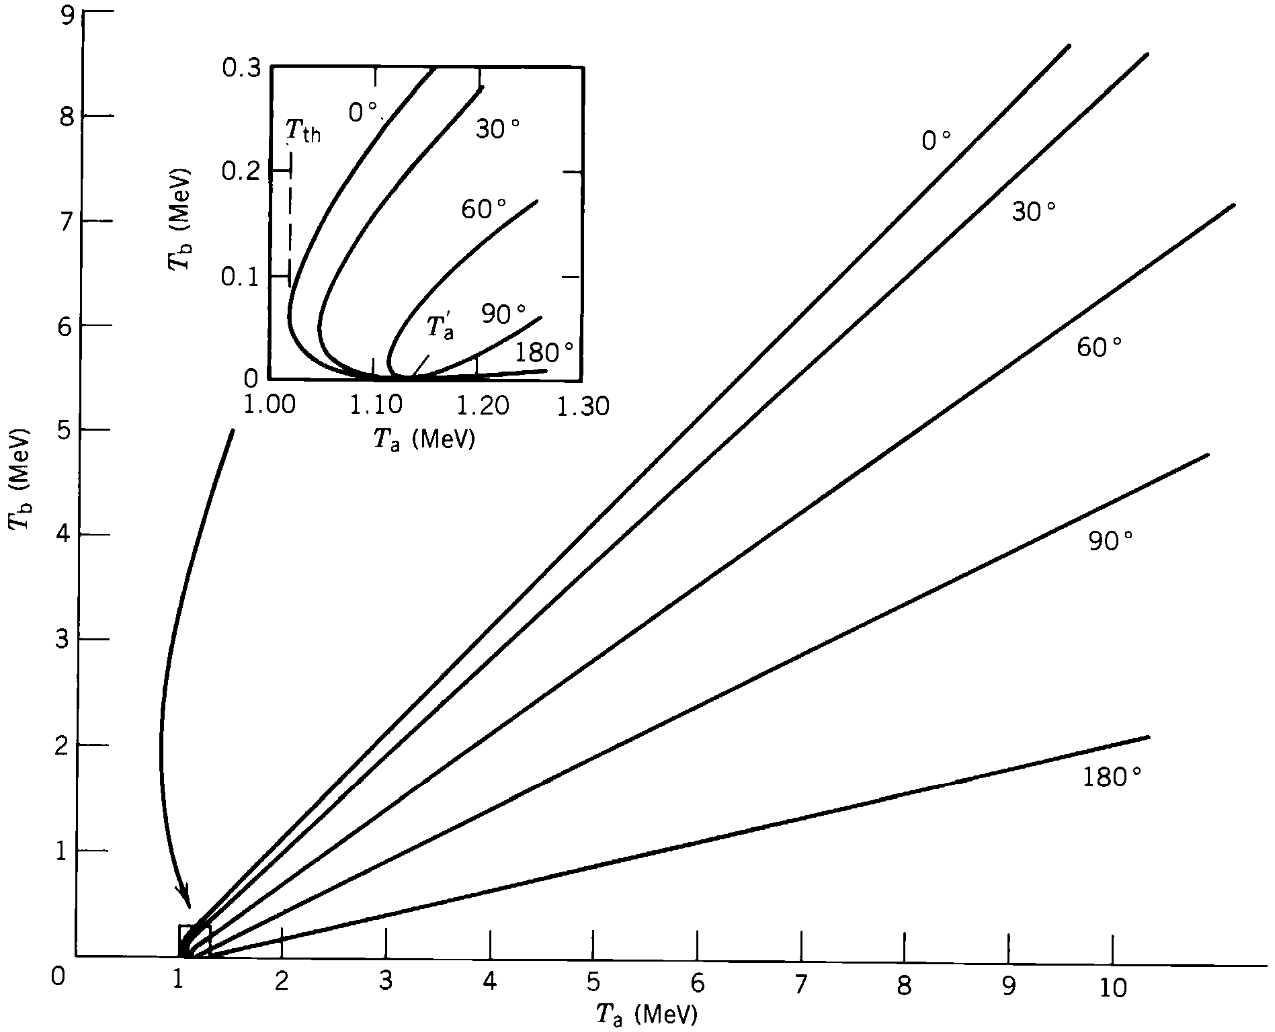
\includegraphics[width=0.70\textwidth]{reac-graph.png}
	\caption{$ T_{\mathrm{b}} $ vs $ T_{\mathrm{b}} $ at various outgoing angles for $ \ch{^3H} \left( p,n \right) \ch{^3He} $.}
	\label{reac-graph}
\end{figure}

\paragraph{Stati eccitati}

È possibile che il nuclide $ \mathrm{Y} $ sia prodotto in uno stato eccitato $ \mathrm{Y}^* $; in tal caso, si vede che il $ Q $-value diminuisce a causa dell'excitation energy $ E_{\text{ex}} $:
\begin{equation}
	Q = Q_0 - E_{\text{ex}}
	\label{eq:6.4}
\end{equation}
dove $ Q_0 $ è relativo alla reazione che produce $ \mathrm{Y} $ nel ground state. È quindi possibile ricostruire lo spettro della specie $ \mathrm{Y} $ calcolando il $ Q $-value a partire da $ T_{\mathrm{a}} $, $ \theta $ (fissati) e $ T_{\mathrm{b}} $ (misurato), il che è possibile invertendo l'Eq. \ref{eq:6.2}:
\begin{equation}
	Q = \left( 1 + \frac{M_{\mathrm{b}}}{M_{\mathrm{Y}}} \right) T_{\mathrm{b}} - \left( 1 - \frac{M_{\mathrm{a}}}{M_{\mathrm{Y}}} \right) T_{\mathrm{a}} - 2 \sqrt{\frac{M_{\mathrm{a}}}{M_{\mathrm{Y}}} \frac{M_{\mathrm{b}}}{M_{\mathrm{Y}}} T_{\mathrm{a}} T_{\mathrm{b}}} \cos \theta
	\label{eq:6.5}
\end{equation}
Solitamente si raggiunge una sufficiente accuratezza utilizzando i numeri atomici al posto delle masse nucleari, specialmente per $ \theta \approx \frac{\pi}{2} $ (si annulla l'ultimo termine).

\paragraph{Cross-section}

Si consideri un projectile beam d'intensità $ \Phi_0 $ (particelle al secondo) diretto su uno strato sottile di nuclei target con spessore $ s $: a causa delle interazioni coi targets, il projectile beam risulta attenuato a seguito del passaggio nello strato sottile, con un'intensità risultante $ \Phi_{\text{f}} $. La frazione di particelle incidenti che reagiscono è funzione della densità numerica di targets $ n_{\text{t}} $ e dalla cross-section $ \sigma $ della reazione:
\begin{equation}
	d\Phi = - \Phi n_{\text{t}} \sigma dx
	\quad \Rightarrow \quad
	\Phi_0 - \Phi_{\text{f}} = \Phi_0 \left( 1 - e^{- n_{\text{t}} \sigma s} \right) \approx \Phi_0 n_{\text{t}} \sigma s
	\label{eq:6.6}
\end{equation}

\paragraph{Trattazione semiclassica}

Classicamente, si può pensare ai nuclidi come sfere rigide che urtano, con vari risultati a seconda del parametro d'impatto $ b $: per $ b \approx R_{\mathrm{X}} $ si ha un urto elastico, per $ b \ll R_{\mathrm{X}} $ ci può essere uno scambio di nucleoni tra i nuclidi, per $ b \approx 0 $ si può arrivare alla formazione di un unico nucleo composto dal nucleo target e da quello incidente.

\section{Reazioni di diffusione e scattering}

Si dicono reazioni di diffusione o di scattering quelle reazioni in cui $ \mathrm{b} = \mathrm{a} $ (o suoi stati eccitati). Si parla di \textit{scattering elastico} per le reazioni $ \mathrm{A} \left( \mathrm{a},\mathrm{a} \right) \mathrm{A} $, di \textit{scattering inelastico} negli altri casi.\\
Lo scattering nucleare elastico presenta delle somiglianze col problema ottico della diffrazione da disco opaco: un nucleo è un forte assorbitore di nucleoni, da cui l'analogia col disco opaco. Come si vede in Fig. \ref{opdisk}, la diffrazione da disco opaco circolare, dunque con bordo ben definito, risulta in un pattern con massimi e minimi approssimativamente equispaziati e d'intensità decrescente, con il primo minimo a $ \theta \approx \frac{\lambda}{R} $ ($ \lambda $ lunghezza d'onda incidente, $ R $ raggio del disco).

\begin{figure}[!b]
	\centering
	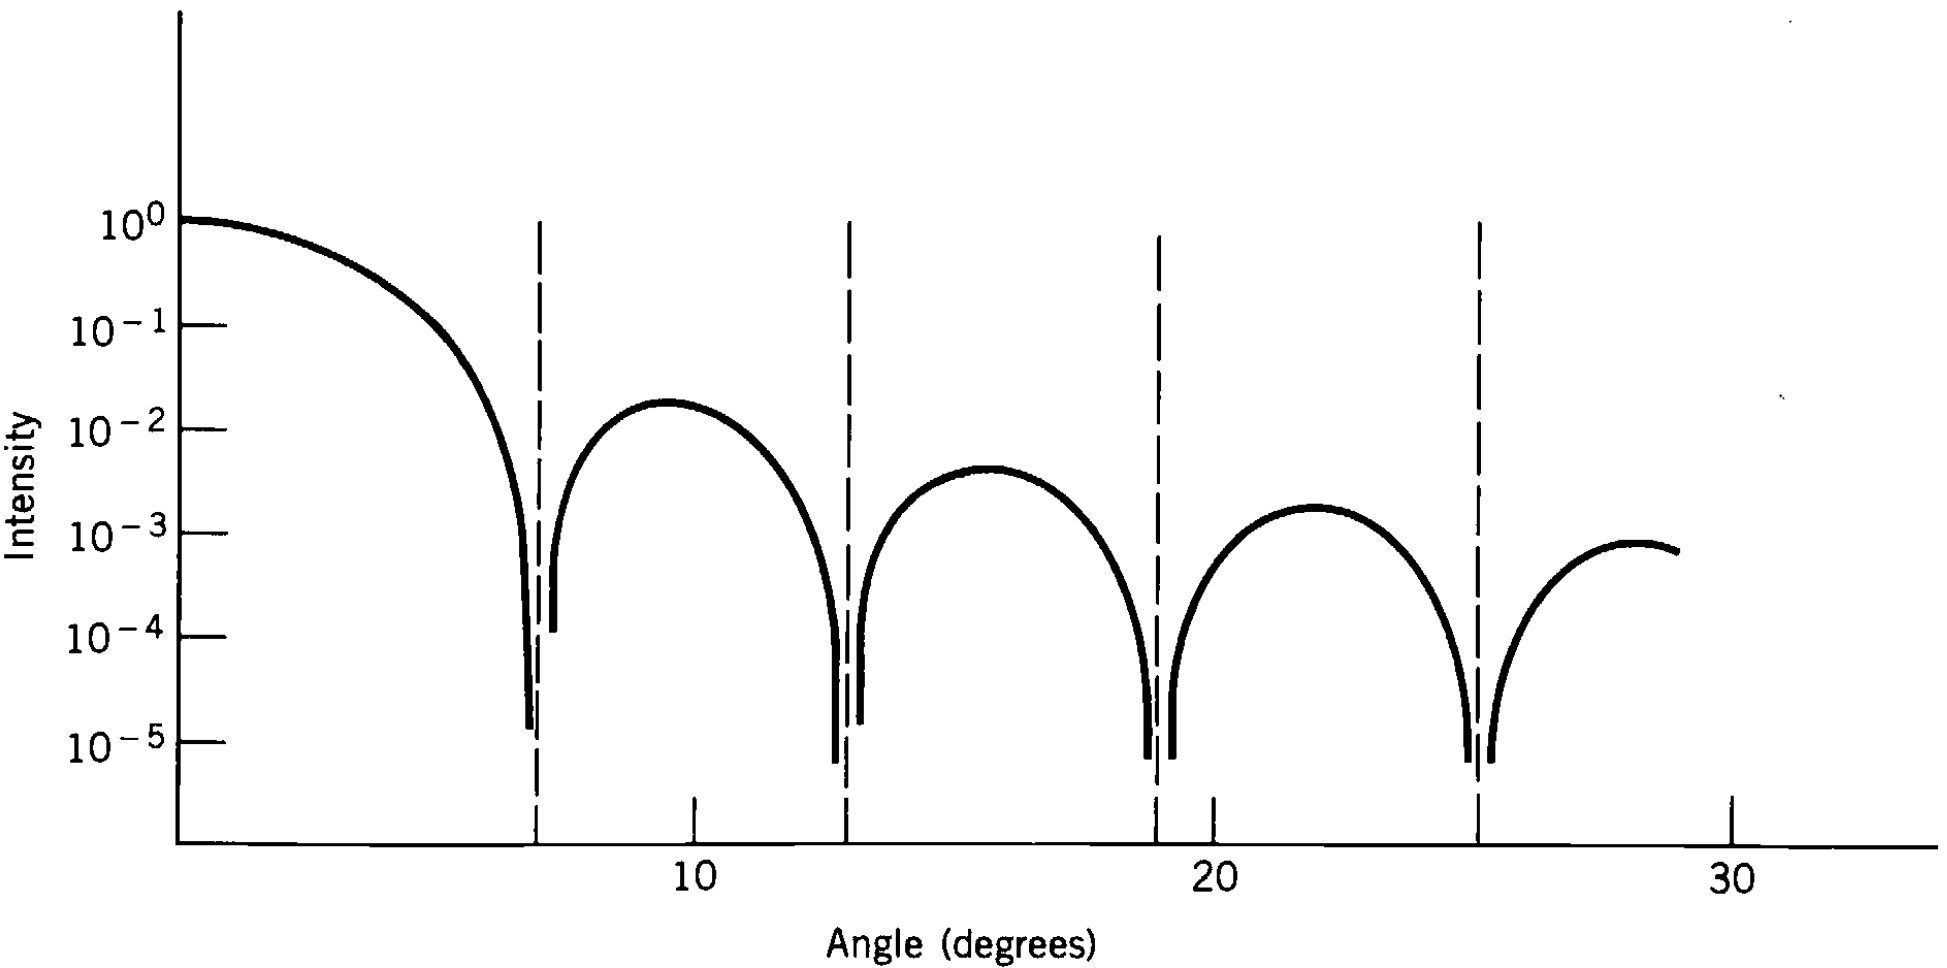
\includegraphics[width=0.70\textwidth]{opdisk.png}
	\caption{Diffraction pattern of light incident on an opaque circular disk.}
	\label{opdisk}
\end{figure}

\begin{figure}[H]
	\centering
	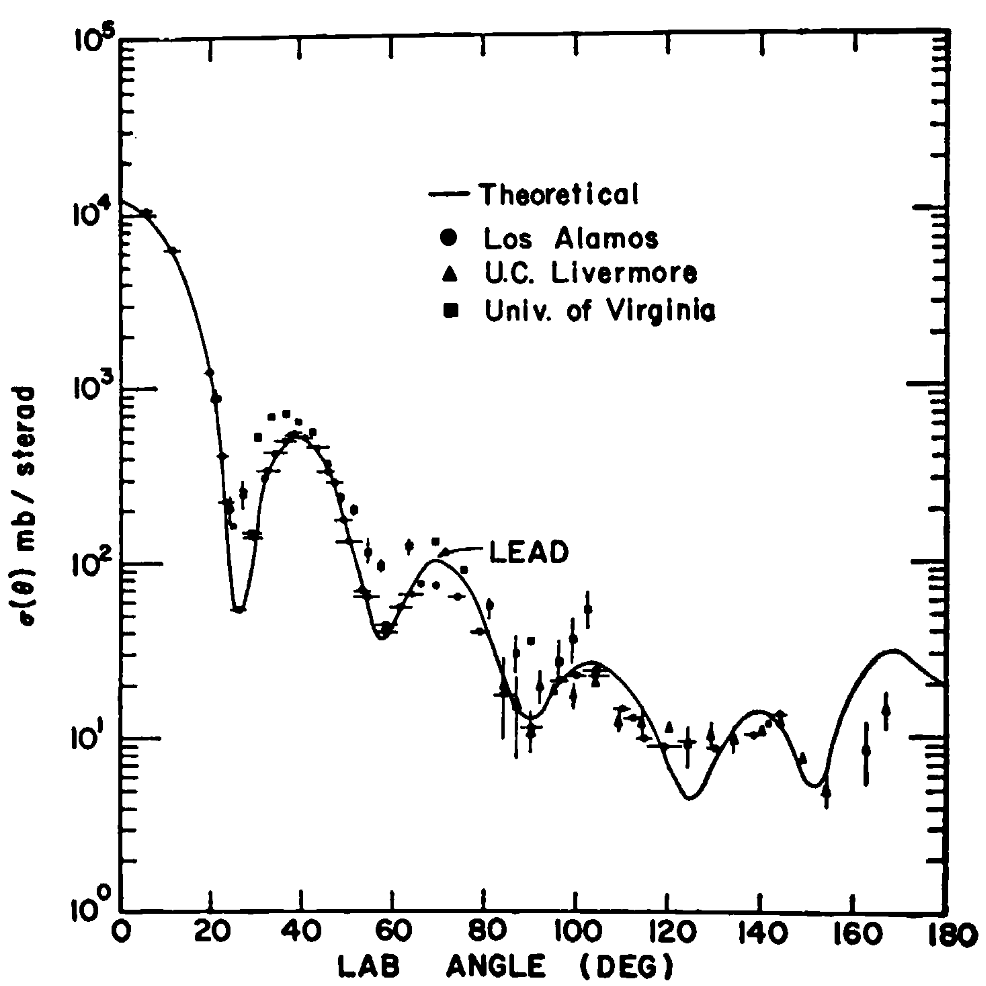
\includegraphics[width=0.70\textwidth]{neutron-scatt.png}
	\caption{Neutron scattering at $ 14\mev $ from $ \ch{^{208}Pb} $.}
	\label{neutron-scatt}
\end{figure}
\begin{figure}[H]
	\centering
	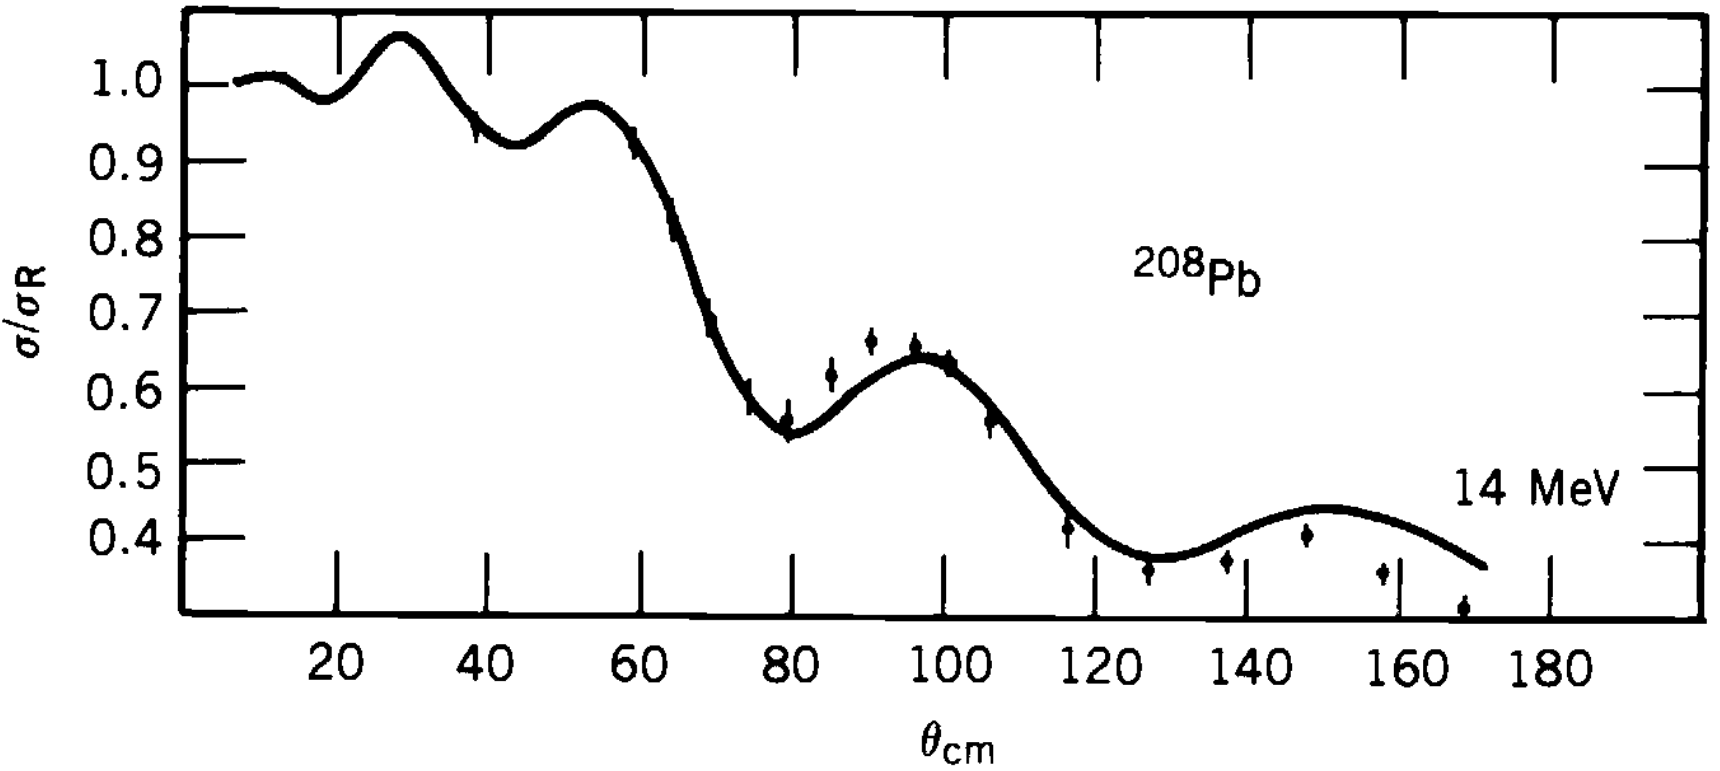
\includegraphics[width=0.70\textwidth]{proton-scatt.png}
	\caption{Proton scattering at $ 14\mev $ from $ \ch{^{208}Pb} $.}
	\label{proton-scatt}
\end{figure}

Nel caso di particelle cariche, si deve considerare la presenza, oltre che dello scattering nucleare, dello scattering coulombiano. Come si vede in Fig. \ref{neutron-scatt}, lo scattering di neutroni, che non subiscono l'interazione coulombiana, segue quasi esattamente il pattern diffrattivo in Fig. \ref{opdisk}, con la differenza che i minimi non vanno a zero dato che la superficie nucleare ha una certa diffusività. Lo scattering di protoni, invece, ha un comportamento diverso: dalla Fig. \ref{proton-scatt} si nota che il comportamento diffrattivo si ha solo per angoli grandi; ad alte energie, invece, l'interazione coulombiana diventa trascurabile.\\
Un'applicazione dello studio dello scattering nucleare è la stima del raggio nucleare: sebbene i valori esatti dipendano dallo specifico potenziale utilizzato per analizzare lo scattering, i risultati sono consistenti con $ R = R_0 A^{1/3} $, con $ R_0 = 1.25\fm $, oltre a mostrare la diffusività della superficie nucleare.

\begin{figure}[!b]
	\centering
	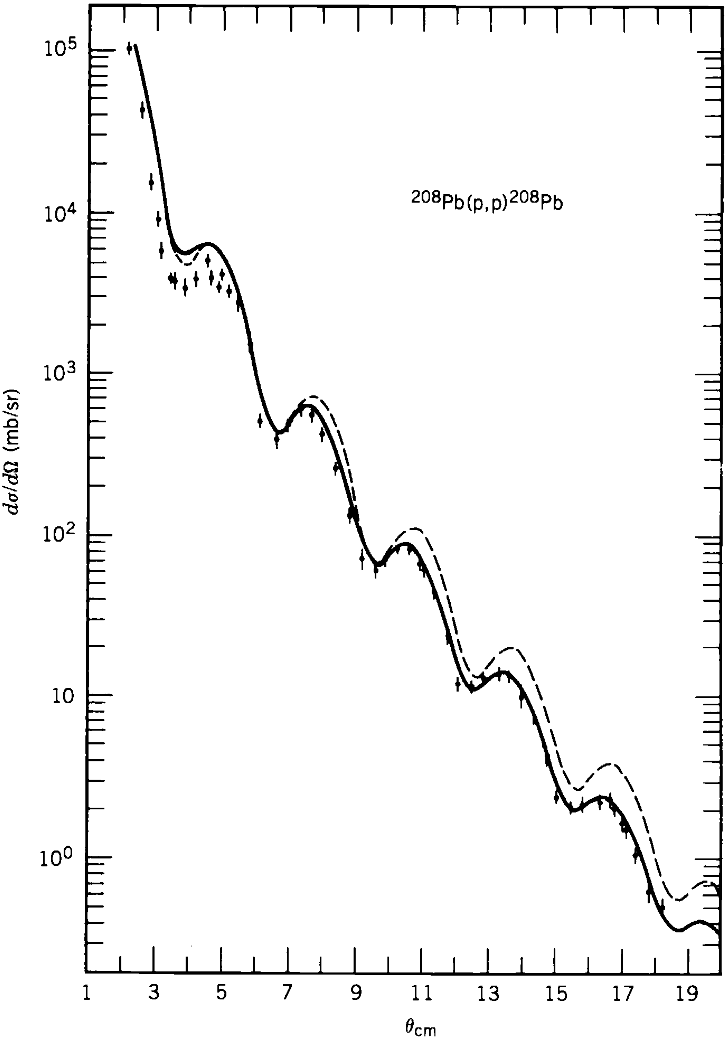
\includegraphics[width=0.75\textwidth]{he-proton-scatt.png}
	\caption{Proton scattering at $ 1050\mev $ from $ \ch{^{208}Pb} $.}
	\label{he-proton-scatt}
\end{figure}

\section{Reazioni dirette ed indirette}

Un'ulteriore classificazione delle reazioni non-scattering è data dalla durata della reazione:
\begin{enumerate}
	\item reazioni dirette, che avvengono in un tempo breve rispetto al tempo di transito del proiettile nel target ($ \sim 10^{-22}\,\text{s} $):
		\begin{itemize}
			\item reazioni di stripping: uno o più nucleoni sono trasferiti dal proiettile al target;
			\item reazioni di pick-up: uno o più nucleoni sono trasferiti dal target al proiettile (es.: $ \left( p,d \right) $, $ \left( n,d \right) $, $ \left( d,\ch{^3H} \right) $, $ \left( d,\ch{^3He} \right) $);
			\item reazioni di knock-out: il proiettile strappa uno o più nucleoni dal target, ma non li assorbe;
		\end{itemize}
	\item reazioni indirette, che avvengono tramite la formazione di uno stato intermedio, detto \textit{nucleo composto}, che dopo un certo tempo decade e produce le particelle finali:
		\begin{itemize}
			\item canale elastico: $ \mathrm{a} + \mathrm{A} \rightarrow \mathrm{C}^* \rightarrow \mathrm{a} + \mathrm{A} $;
			\item canale inelastico: $ \mathrm{a} + \mathrm{A} \rightarrow \mathrm{C}^* \rightarrow \mathrm{a} + \mathrm{B} $;
			\item reazione nucleare: $ \mathrm{a} + \mathrm{A} \rightarrow \mathrm{C}^* \rightarrow \mathrm{b} + \mathrm{B} $;
			\item cattura radiativa: $ \mathrm{a} + \mathrm{A} \rightarrow \mathrm{C}^* \rightarrow \gamma + \mathrm{C} $.
		\end{itemize}
\end{enumerate}
La separazione tra le due classi non è ben definita: in genere, si dicono indirette le reazioni che impiegano più di $ 1\,\mu\text{s} $.\\
Le reazioni dirette avvengono quando la particella incidente è abbastanza energetica da avere una lunghezza d'onda di de Broglie $ \lambda \sim 1\fm $ (es.: un nucleone da $ 20\mev $), interagendo dunque con singoli nucleoni alla periferia del nucleo: si parla infatti di \textit{peripheral processes}. La particella risultante è generalmente emessa in avanti, ovvero ad angoli piccoli rispetto alla direzione della particella incidente.

\subsection{Reazioni di stripping}

Le reazioni di stripping più semplici sono quelle indotte dal deuterio $ d \equiv \ch{^2H} $ (binding energy $ 2.2\mev $):
\begin{equation*}
	d + \ch{X}(A,Z) \rightarrow p + \ch{X}(A+1,Z)
	\qquad \qquad
	d + \ch{X}(A,Z) \rightarrow n + \ch{X}(A,Z+1)
\end{equation*}
È possibile trattare in maniera semiclassica tale reazione, ignorando gli spin delle particelle. Si consideri una particella incidente con momento $ \ve{p}_a $ che determina una particella in uscita di momento $ \ve{p}_b $: il nucleo residuale, composto dal nucleo iniziale più il nucleone scambiato, ha quindi un momento di recoil $ \ve{p} = \ve{p}_a - \ve{p}_b $. In un processo diretto è possibile assumere che il trasferimento di momento sia istantaneo e che il nucleone scambiato venga posto in un orbitale nucleare con $ \ell \approx \frac{1}{\hbar} Rp $, dove $ R $ è il raggio del nuclide (peripheral process):
\begin{equation*}
	p^2 = p_a^2 + p_b^2 - 2 p_a p_b \cos \theta = \left( p_a - p_b \right)^2 + 2 p_a p_b \left( 1 - \cos \theta \right)
\end{equation*}
Assumendo $ p_a \approx p_b \equiv p_0 $, si trova:
\begin{equation}
	\ell = \frac{2}{\hbar} R p_0 \sin \frac{\theta}{2}
	\label{eq:6.7}
\end{equation}
Ad esempio, si consideri la reazione $ \ch{^{90}Zr} \left( d,p \right) \ch{^{91}Zr} $: essa $ Q = 5\mev $, dunque un deuterone incidente di $ 5\mev $ produce un protone in uscita di $ 10\mev $, al meno di eccitazioni di $ \ch{^{91}Zr} $.
Come si vede in Fig. \ref{zr-spec}, i picchi nello spettro di protoni della reazione identificano vari stati eccitati del $ \ch{^{91}Zr} $ che vengono popolati dalla reazione. Dallo studio degli angoli a cui vengono emessi i protoni (Fig. \ref{zr-ang}), ed in particolare dei massimi della distribuzione angolare di protoni, si posso determinare i numeri quantici $ \ell $ dei neutroni trasferiti e, di conseguenza, delle shell che essi occupano nei vari stati eccitati.

\begin{figure}[H]
	\centering
	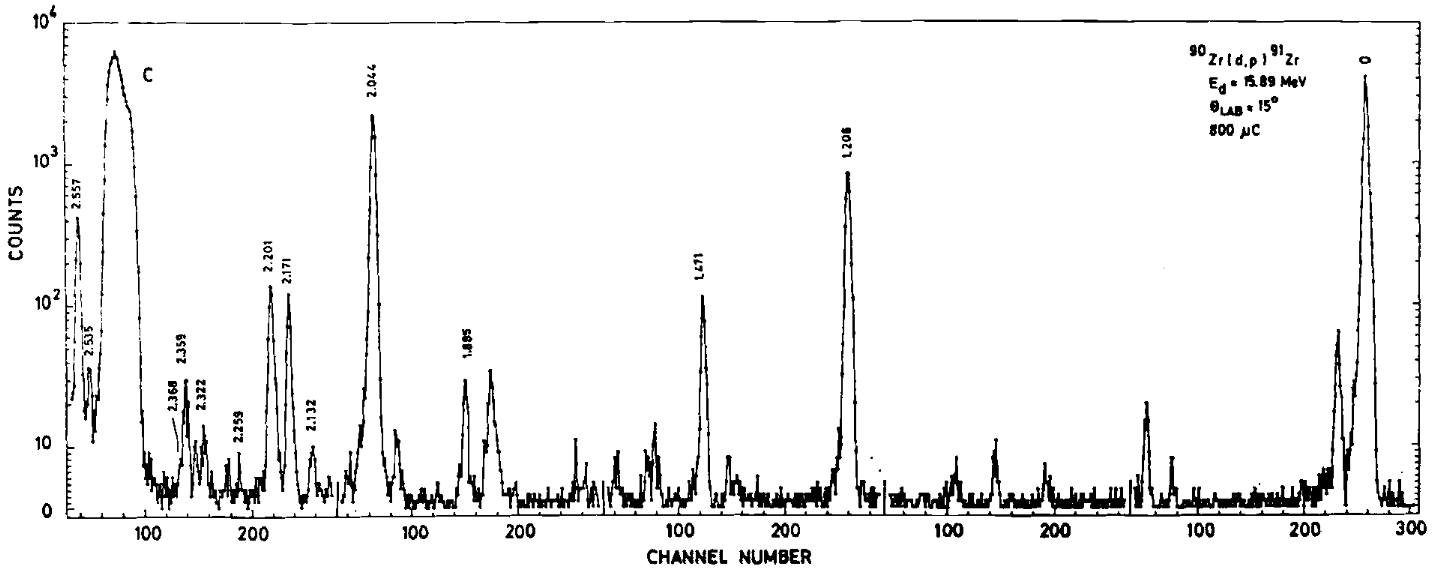
\includegraphics[width=0.75\textwidth]{zr-spec.png}
	\caption{Proton spectrum from $ \ch{^{90}Zr} \left( d,p \right) \ch{^{91}Zr} $.}
	\label{zr-spec}
\end{figure}

\begin{figure}[H]
	\centering
	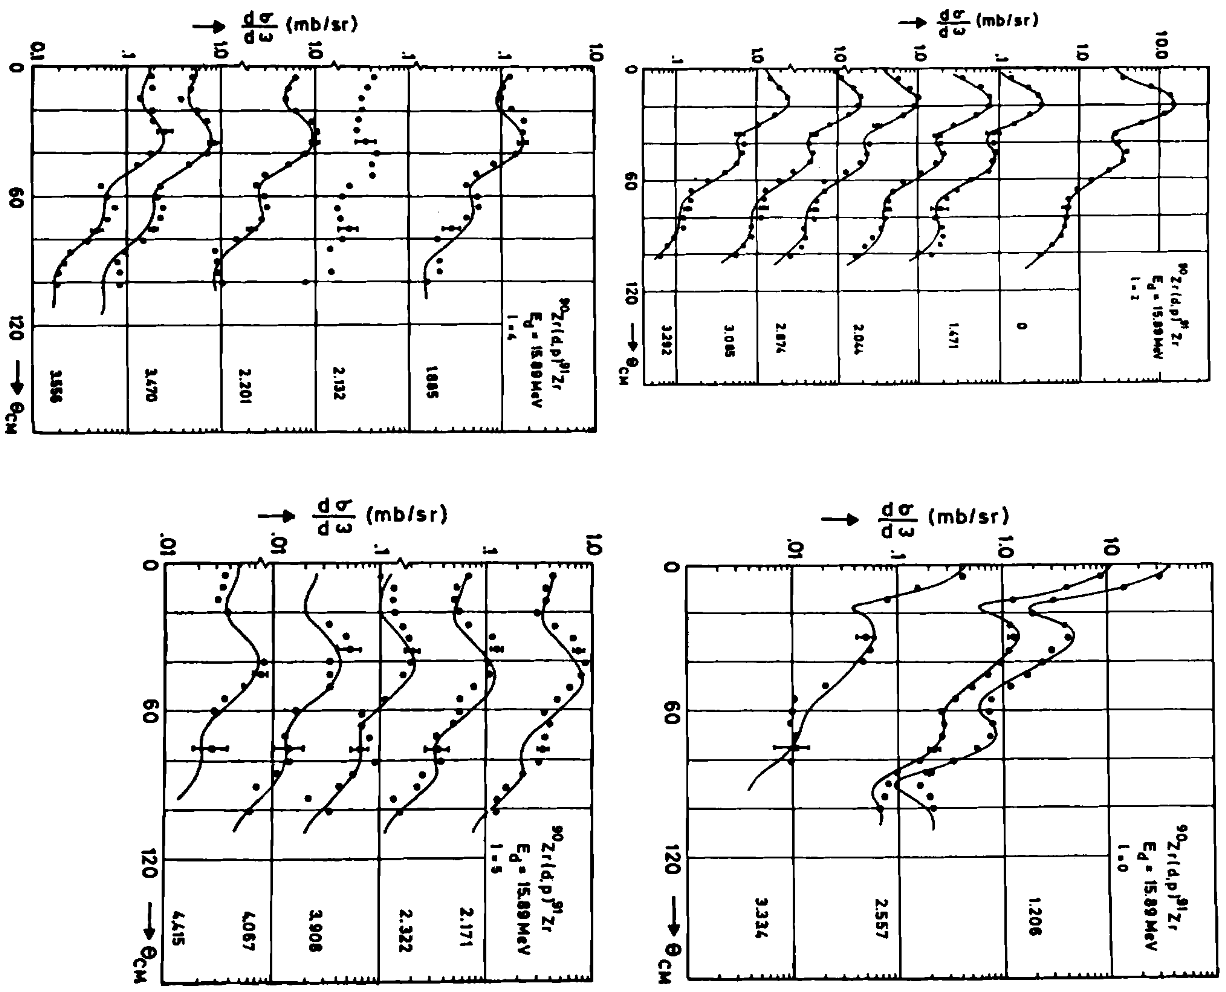
\includegraphics[width=0.60\textwidth, angle=90]{zr-ang.png}
	\caption{Angular distributions for $ \ch{^{90}Zr} \left( d,p \right) \ch{^{91}Zr} $.}
	\label{zr-ang}
\end{figure}

\subsection{Reazioni di nucleo composto}

Si consideri una particella proiettile che penetra il nucleo target con un parametro d'impatto piccolo rispetto al raggio nucleare: ciò genera una serie di collisioni interne al nucleo composto così formato, con un conseguente aumento dell'energia media per nucleone. Le collisioni random che avvengono all'interno del nucleo ripartiscono l'energia incidente tra tutti i nucleoni del sistema proiettile+target secondo una certa distribuzione statistica di energia, dunque c'è una certa probabilità che un nucleone accumuli abbastanza energia per fuggire dal potenziale nucleare, in maniera equivalente ad una molecola in un liquido in evaporazione. Data la natura casuale delle collisioni nel nucleo, le particelle così emesse sono distribuite isotropicamente nello spazio (a differenza delle reazioni dirette che emettono tendenzialmente in avanti) e la loro energia è distribuita secondo una distribuzione maxwelliana.\\
Si vede dunque che le reazioni di nucleo composto possono essere divise in due step: la formazione del nucleo composto ed il suo successivo decadimento, il quale può avere vari decay modes con meccanismi diversi. L'assunzione fondamentale, confermata dai dati sperimentali, è che la probabilità relativa di un certo decay mode è indipendente da come si è formato il nucleo composto, ma determinata soltanto dall'energia totale del sistema.\\
Il modello a nucleo composto funziona bene per proiettili a bassa energia, che hanno una bassa probabilità di fuoriuscire dal nucleo senza subire cambiamenti e senza cessioni di energia, e per target medi e pesanti, che hanno una struttura nucleare abbastanza grande da assorbire tutta l'energia incidente.

\section{Reazioni fotonucleari}

L'analisi dettagliata delle reazioni indotte dai fotoni sui nuclei permette di studiare le eccitazioni collettive di molti nucleoni, andando oltre i modelli di particella singola: queste sono spiegate fenomenologicamente come fluttuazioni di forma o densità del sistema many-body attorno ad uno stato d'equilibrio.\\
La produzione di raggi $ \gamma $ monocromatici è possibile grazie a sorgenti radioattive (es.: $ \ch{^{24}Na} $ e $ \ch{^{60}Co} $, con $ E_{\gamma} \approx 1-3\mev $) e fasci protonici incidenti su litio ($ p + \ch{Li} $ produce raggi $ \gamma $ con $ E_{\gamma} \approx 17\mev $); sorgenti di raggi $ \gamma $ ad energia variabile sono invece basate sull'annichilazione di positroni.\\
Con i fasci ad enegia variabile sono stati ottenuti risultati di precisione sia sulla sezione d'urto totale dell'assorbimento di un fotone dal nucleo, sia sulla \textit{fotoproduzione di neutroni}:
\begin{equation*}
	\gamma + \ch{X}(A,Z)\rightarrow n + \ch{X}(A-1,Z)
\end{equation*}
Questa reazione rappresenta la maggior parte della sezione d'urto totale, dato che la fotoproduzione di protoni è sfavorita dalla barriera coulombiana.

\paragraph{Giant Dipole Resonance}

La cross-section da assorbimento di fotoni è dominata da un'ampia risonanza, nota come \textit{Giant Dipole Resonance} (GDR). Ad esempio, si consideri la cross-section per la fotoproduzione di neutroni da isotopi di \ch{Nd}, riportata in Fig. \ref{gdr-nd}: si vede che la sezione d'urto presenta un massimo per $ E_{\gamma} \approx 15\mev $ ed un andamento a risonanza abbastanza larga. La GDR è osservata per moltissimi nuclei, da quelli leggeri come $ \ch{^3He} $ a quelli pesanti come $ \ch{^{232}Th} $; per nuclei medi e pesanti, l'energia di eccitazione della risonanza può essere stimata come $ E_{\text{GDR}} \approx A^{-1/3} \cdot 80\mev $.

\begin{figure}
	\centering
	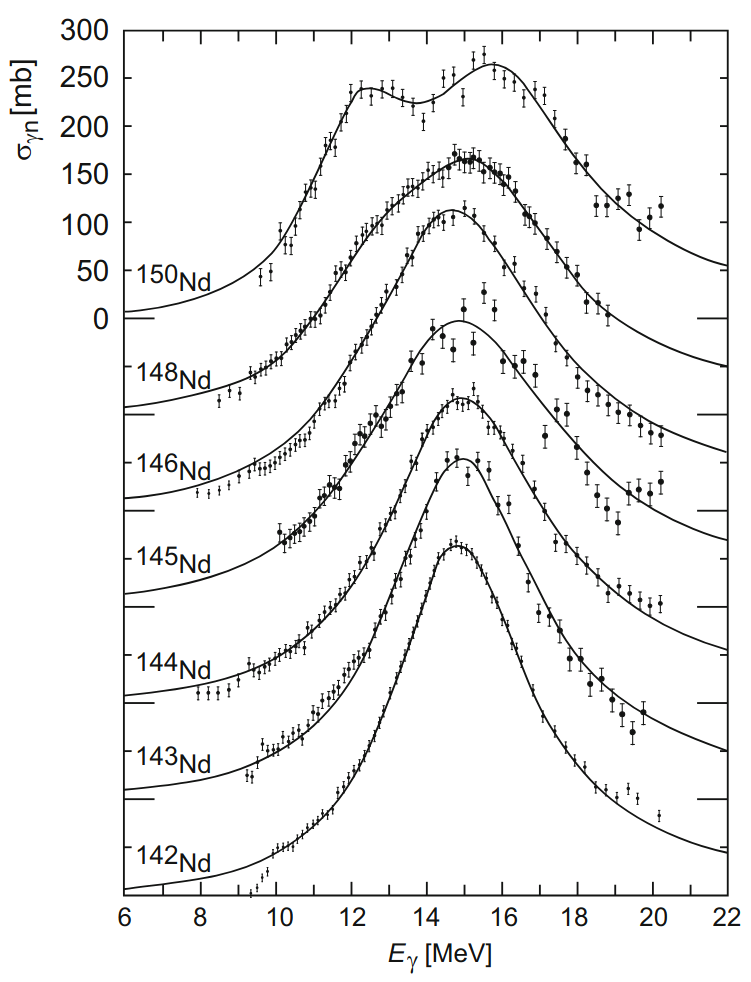
\includegraphics[width=0.70\textwidth]{gdr.png}
	\caption{Cross-section for $ \gamma $-induced emission of neutrons in neodymium isotopes.}
	\label{gdr-nd}
\end{figure}









